% !TeX spellcheck = en_GB
%!TEX root = ../thesis.tex

\chapter{Nonlinear harmonic systems} \label{ch:hb}


\begin{chapterabstract}
	
This chapter is dedicated to modelling physical systems using nonlinear ordinary differential equations (ODEs). Our focus is primarily on systems which behave harmonically in time, typically as a result of periodic driving. We start by demonstrating how a continuous structure (an elastic membrane) gives rise to a set of ODEs. We then introduce the method of harmonic balance -- the primary tool used to treat periodically-driven systems in this thesis, which transforms a set of ODEs into a set of polynomial equations. Solving these, even numerically, is a challenge of its own due to the potentially high number of roots. We use the method of homotopy continuation to find all the solutions of any given system and show that it can solve hitherto intractable nonlinear problems. Finally, we use harmonic balance to look at a simpler, analytically-treatable case to elucidate the elusive phenomenon of nonlinear damping. 

%
\tcblower
%
The material presented in this chapter is largely taken from Ref.~\cite{Kosata_2022a}, dedicated to the software package HarmonicBalance.jl. The package is an integral part of this work and is the subject of Appendix~\ref{app:hb}.
\end{chapterabstract} 

As mentioned in the Introduction (Sec.~\ref{sec:intro_nonlin}), nonlinear ODEs appear across virtually all domains of physics. Before plunging into the details of their solving, let us get an impression of how one obtains a system of ODEs from a physical model.

\section{Example system: A rectangular elastic membrane} \label{sec:hb_membrane_eom}

Here, we analyse a stretched rectangular elastic membrane under the influence of an external force. Specifically, we are interested in its out-of-plane displacement $w \equiv w(x,y,t)$, which is described by the field Lagrangian\footnote{The Lagrangian originates from the kinetic and potential energies of a thin plate subject to large external stretching forces. In this limit, the potential energy is dominated by (nonlinear) strain, while bending can be neglected. For more details, see~\cite{Landau_Lifshitz_7, Ugural}.}
\begin{equation}
\mathcal{L} = \frac{\rho h}{2} \dot{w}^2 - \frac{\bar{\sigma} h}{2} \left(\grad w \cdot \grad w\right) - \frac{\alpha}{4} \left(\grad w \cdot \grad w\right)^2 - f w\,,
\end{equation}
where $\bar{\sigma}$ is the applied stress, $\rho$ the material density and $h$ the thickness of the membrane. The nonlinearity coefficient $\alpha = \frac{E h}{2 (1 - \nu^2)}$, where $E$ and $\nu$ denote Poisson's ratio, respectively. $f \equiv f(x,y,t)$ is the external force.

Employing the Galerkin discretisation method~\cite{Nayfeh_Mook}, we express the displacement $w$ using the normal modes of the linear limit ($\alpha=0$). Each of these modes is characterised by a pair of integers $\vb{j} = (j_1, j_2)$; for a membrane clamped at $x = 0, L_x$ and $y = 0, L_y$,
\begin{equation} \label{eq:hb_rect_modes}
\phi_{\vb{j}}(x,y) = \sin(\frac{j_1 \pi x}{L_x}) \sin(\frac{j_2 \pi y}{L_y})\,.
\end{equation}
These modes are used as a basis to decompose $w$ such that each mode is factorised into its spatial shape $\phi_{\vb{j}}(x,y)$ (unitless) and its amplitude $u_{\vb{j}}(t)$ (units of length),
\begin{equation}
w(x,y,t) = \sum_{\vb{j}} u_{\vb{j}}(t) \phi_{\vb{j}}(x,y)\,.
\end{equation}
Note that this approach is exact where the sum over $\vb{j}$ goes to infinity. The resulting Lagrange's equations of motion for each $u_{\vb{j}}(t)$ read, dropping the brackets,
\begin{multline} \label{eq:hb_rect_eom}
\left( \rho h \int_S \phi_{\vb{j}}^2 dS \right) \ddot{u}_{\vb{j}} + \left(\bar{\sigma} h \int_S \grad \phi_{\vb{j}} \cdot \grad \phi_{\vb{j}} dS \right) u_{\vb{j}} + \alpha \sum_{\vb{k} \vb{l} \vb{m}} C_{\vb{j} \vb{k} \vb{l} \vb{m}} u_{\vb{k}} u_{\vb{l}} u_{\vb{m}}\\ = \int_S f \phi_{\vb{j}} dS\,,
\end{multline}
with $ \int_S dS = \int_{0}^{L_x} dx \int_0^{L_y} dy$ and $C_{\vb{j} \vb{k} \vb{l} \vb{m}}$ a tensor,
\begin{equation} \label{eq:hb_rect_C}
C_{\vb{j} \vb{k} \vb{l} \vb{m}} = \int_S dS \left(\grad \phi_{\vb{j}} \cdot \grad \phi_{\vb{k}}  \right)  \left(\grad \phi_{\vb{l}} \cdot \grad \phi_{\vb{m}}  \right)\,.
\end{equation}
The linear part of Eq.~\eqref{eq:hb_rect_eom} gives us the natural frequency of each mode,
\begin{equation}
\omega_{\vb{j}}= \sqrt{\frac{\bar{\sigma} \int_S \grad \phi_{\vb{j}} \cdot \grad \phi_{\vb{j}}\, dS}{ \rho \int_S \phi_{\vb{j}}^2 \,dS}} = \pi \sqrt{ \frac{\bar{\sigma}}{\rho}  \left(\frac{j_1^2}{L_x^2} + \frac{j_2^2}{L_y^2} \right)} \,.
\end{equation}
The nonlinear part consists of terms involving one or more modes -- these are sometimes called \textit{self-} and \textit{cross-nonlinearities}, respectively. The self-nonlinearity of each mode, 
\begin{equation}
C_{\vb{j} \vb{j} \vb{j} \vb{j}} = \frac{9 (j_1 L_x)^4 + 2 (j_1 j_2 L_x L_y)^2 + 9 (j_2 L_y)^4}{64 (L_x L_y)^3} > 0 \,,
\end{equation}
gives a term cubic in $u_{\vb{j}}$ in Eq.~\eqref{eq:hb_rect_eom}. Every single mode thus has a cubic nonlinearity: such a system is known as a \textit{Duffing} or a \textit{Kerr oscillator}. The cross-nonlinearities are slightly harder to evaluate, since all index permutations must be considered in the summation in Eq.~\eqref{eq:hb_rect_eom}. We leave the explicit treatment of these to Sec.~\ref{sec:hb_mem_driven}.

\subsubsection{Selection rules for nonlinear interactions}

In this specific case, not all possible mode coupling terms appear. Having analytical functions for $\phi_{\vb{j}}$ at our disposal, we may identify the non-vanishing tensor components of $C_{\vb{j} \vb{k} \vb{l} \vb{m}}$. Considering Eq.~\eqref{eq:hb_rect_C} with the mode shapes given in Eq.~\eqref{eq:hb_rect_modes}, we have two spatial integrals, each over a product of four cosines. For $C_{\vb{j} \vb{k} \vb{l} \vb{m}}$ to not vanish, each of the products must give a contribution constant in $x$ and $y$, i.e.,
\begin{equation}
j_1 \pm k_1 \pm l_1 \pm m_1 = 0  \quad \text{and} \quad j_2 \pm k_2 \pm l_2 \pm m_2 = 0 
\end{equation}
must hold for one choice of the $\pm$ signs.

This completes our description of the equations of motion -- now, a concrete forcing term $f$ must be chosen, which will typically be a periodic function of time. We therefore introduce the method of harmonic balance, which addresses the time dependence of our problem.

\section{The method of harmonic balance} \label{sec:hb}
Harmonic balance is a method to treat harmonically-driven nonlinear systems, i.e., dynamical systems governed by equations of motion where all explicitly time-dependent terms are harmonic. In the exposition here, we will assume a general nonlinear system of $N$ second-order ODEs\footnote{Second-order ODEs based on the harmonic oscillator represent the vast majority of expected use cases. However, the methods described in this work are applicable to arbitrary ODE orders~\cite{Richards}.} with real variables $x_i(t)$, where $i = 1,2,\ldots,N$ and time $t$ as the independent variable,
\begin{equation} \label{eq:hb_general_ode}
\vb{G}(\vb{x}(t), t)=0\:.
\end{equation}
The vector $\vb{x}(t) = (x_1(t), ..., x_N(t))^{\text T}$ fully describes the state of the system.  Physically, $\vb{x}(t)$ represents the amplitudes of either point-like or collective oscillators (e.g., mechanical resonators, voltage oscillations in $RLC$ circuits, an oscillating electrical dipole moment, or modes of an elastic membrane). $\textbf{G}(\textbf{x}(t),t)$ typically depends on both $\vb{x}(t)$ and its time derivatives. We assume it can be decomposed into a sum of $L$ periodic terms\footnote{We omit the time dependence where this is clear from the context.},
\begin{equation} \label{eq:hb_G}
\vb{G}(\vb{x}, t) = \vb{g}_0(\vb{x}) + \sum_{l=1}^L \vb{g}_{l}(\vb{x}) \cos(\omega_l t + \phi_l)\,,
\end{equation}
with vector fields $\vb{g}_l(\vb{x})$.  The field $\vb{g}_0$ describes static properties of the system while $\vb{g}_{l\neq0}$ account for explicit time-dependence, typically induced by one or more sources of periodic driving and/or parameter modulation with frequencies $\{\omega_l\}$ and phases $\{\phi_l\}$. In Table~\ref{table:hb_terms}, we list several examples of terms commonly constituting Eq.~\eqref{eq:hb_general_ode}. 

\begin{table}[t] 
	\centering
	\caption{Examples of terms occurring in Eq.~\eqref{eq:hb_general_ode} and their origins. The rightmost column shows the frequency conversion taking place, assuming two variables $x_i$, $x_j$, oscillating at frequencies $\omega_i$, $\omega_j$ (for example, $\omega_i \rightarrow 2\omega_i$ means that oscillating at frequency $\omega_i$ leads to additional oscillations at frequency $2\omega_i$).}
	\label{table:hb_terms}
	\begin{tabular}{ |c|c|c| } 
		\hline
		term in $F_i(\vb{x}, t)$ & physical mechanism & frequency conversion \\ \hline
		$x_i$ & natural response (spring constant) & - \\
		$x_j$ & mode coupling & - \\
		$\dot{x}_i$ & damping/gain & -\\
		$\dot{x}_j$ & dissipative coupling & -\\
		$\cos(\omega_d t)$ & external drive (frequency $\omega_d$) & -\\
		$x_i^2$ & Pockels coefficient & $\omega_i \rightarrow 2\omega_i$ \\ 
		$x_i^3$ & Kerr (Duffing) coefficient & $\omega_i \rightarrow 3 \omega_i$ \\ 
		$x_i^2 \dot{x}_i$ & nonlinear damping & $\omega_i \rightarrow 3 \omega_i$\\ 
		$x_i \cos(\omega_{\rm p} t)$ & parametric drive (frequency $\omega_{\rm p}$) & $\omega_i \rightarrow \omega_i \pm \omega_{\rm p}$\\
		$x_j x_i $ & nonlinear mode interactions & $\omega_i \rightarrow \omega_i \pm \omega_j$\\ 
		\hline
	\end{tabular}
\end{table}

Note that in a linear system, $\vb{G}(\vb{x}, t)$ can be written as $\vb{G}(\vb{x}, t)= \ddot{\vb{x}} + M(t) \vb{x}+ \textbf{b}(t)$, where the matrix $M(t)$ contains spring constants and linear couplings, while $\vb{b}(t)$ is a vector of external forces. Diagonalising $M(t)$ then yields the so-called \textit{normal modes} of the system. While the notion of normal modes does not directly apply in a nonlinear system, they often constitute a convenient basis choice for a perturbative treatment.

\subsection{The harmonic ansatz}\label{sec:harm_exp}

For sufficiently long times (i.e.,~after any transient responses have disappeared), the solutions 
of Eq.~\eqref{eq:hb_general_ode} are expected to appear as a sum over harmonics. Let us illustrate this point using the example of driven harmonic oscillators. In this simple case, Eqs.~\eqref{eq:hb_general_ode} and \eqref{eq:hb_G} take the form
%
\begin{equation} \label{eq:shos}
\ddot{\vb{x}}(t) + M \vb{x}(t) = \vb{F} \cos(\omega_d t)\,,
\end{equation}
%
where we assumed a constant vector $\vb{F}$ and drive frequency $\omega_d$.	The standard method to solve for the steady states is to Fourier-transform both sides of Eq.~\eqref{eq:shos}. The resulting equations give an exact solution for $\vb{x}(t)$ in terms of its Fourier coefficients,
%
\begin{equation} \label{eq:ft_x}
\tilde{\vb{x}}(\omega) = (M - \omega^2 \mathbb{1})^{-1} \vb{F} \left[\delta(\omega + \omega_d) + \delta(\omega - \omega_d)\right] / 2\;,
\end{equation}
%
where $\tilde{\vb{x}}(\omega) = \int_{-\infty}^{+\infty} \vb{x}(t) e^{i\omega t}\: dt$ and $\delta(z-z_0)$ is the Dirac delta function of $z$ centred at $z_0$. This procedure is effective because in the Fourier domain, the l.h.s.~of Eq.~\eqref{eq:shos} becomes diagonal (i.e., it involves a single frequency) while the applied drive reduces to a Dirac delta function centred at $\omega=\omega_d$. We can thus select a single frequency out of the continuous space of all frequencies for which the solution is nonvanishing. Furthermore, due to the linear superposition principle, responses to arbitrary driving terms can be constructed from the solution in Eq.~\eqref{eq:ft_x}.

The same task becomes intractable if nonlinear terms are introduced. Nonlinearities facilitate \textit{frequency conversion} by coupling different harmonics of the system, rendering $\vb{G}(\vb{x},t)$ non-diagonal in Fourier space. As an example, let us consider a single driven Duffing oscillator~\cite{Lifshitz_2008}, whose equation of motion reads
%
\begin{equation} \label{eq:duff_basic}
\ddot{x}(t) + \omega_0^2 x(t) + \alpha x^3(t) = F \cos(\omega_d t) \:.
\end{equation}
%
where $\omega_0$ is the natural frequency, $\alpha$ is the nonlinear coefficient, $F$ is the drive amplitude, and $x$ is now a scalar.
The nonlinear (Duffing) term in Fourier space reads
%
\begin{equation} \label{eq:duffingFT}
\alpha \int x^3(t) e^{-i\omega t} \: dt = \alpha \int_{-\infty}^{+\infty} \tilde{x}(\omega')\tilde{x}(\omega'')\tilde{x}(\omega''') \delta(\omega'''+\omega''+\omega'-\omega) \: d\omega' \: d\omega'' \: d\omega''' \,,
\end{equation}
%
coupling all combinations of four harmonics that sum to zero. This results in frequency conversion processes known as four-wave mixing, which here convert, to lowest order, the driven oscillation at frequency $\omega_d$ to frequency $3\omega_d$; four-wave mixing manifests as off-diagonal terms in Fourier space. The frequency conversion subsequently propagates through the entire spectrum, generating an infinite number of Fourier components. A nonlinearity thus precludes a closed-form solution of the problem in Fourier space; this is a common trait of nonlinear physical systems; see Table~\ref{table:hb_terms} for examples of frequency-converting effects.

A serviceable approach to numerically approximate the harmonics of a driven nonlinear system involves truncating the spectrum  $\tilde{\vb{x}}(\omega)$ to a finite set of frequencies~\cite{Guckenheimer_Holmes}. The idea of truncation in Fourier space is at the core of several widely-used methods, such as harmonic balance~\cite{Krack_2019, Luo_2012}, the rotating-wave approximation~\cite{Gardiner2004}, the van der Pol transformation~\cite{Rand_2005} in combination with Krylov-Bogoliubov averaging~\cite{Nayfeh_2008}, Magnus expansion~\cite{Mikami_2016, Eckardt_2015}, secular perturbation theory~\cite{Lifshitz_2008}, and also appears in the contemporary concept of Floquet engineering~\cite{Rudner_2020, Goldman_2014}. We implement the approach of harmonic balance using a \textit{harmonic ansatz}~\cite{Sarrouy_2011, Guskov_2007}
%
\begin{equation} \label{eq:hb_ansatz}
x_i(t) = \sum_{j=1}^M u_{i,j}  (T)  \cos(\omega_{i,j} t)+ v_{i,j} (T) \sin(\omega_{i,j} t) \,,
\end{equation}
%
where the sum runs over the finite set of desired frequencies $\{\omega_{i,j}\}$ describing the coordinate $x_i$. Here, $T$ represents a "slow time" -- a timescale that is much slower than the oscillations in the system ($T\gg 2\pi/\min \{\omega_j\}$).
Equation~\eqref{eq:hb_ansatz} represents an attempt to capture the dynamics of the system using a discrete set of real functions $\{u_{i,j}(T),v_{i,j}(T)\}$, which we call the \textit{harmonic variables}, while the fast oscillations are accounted for by the sine/cosine terms. Note that this ansatz would be exact if the set of frequencies $\{\omega_{i,j}\}$ covered all real numbers. Generally, it is not straightforward to identify the relevant frequencies $\{\omega_{i,j}\}$. A good starting point is the frequencies of any external drives, combined with the frequency conversions presented in Table~\ref{table:hb_terms}. Alternatively, one can pick the highest-weight discrete Fourier components in a time trace obtained numerically or from experimental data.

Plugging the harmonic ansatz \eqref{eq:hb_ansatz} into the ODE \eqref{eq:hb_general_ode}, we obtain equations governing pairs of harmonic variables $(u_{i,j}, v_{i,j})$ by extracting the coefficients of the respective sines and cosines from both sides. This procedure can be formalised as
\begin{equation} \label{eq:hb_int}
\bar{\vb{G}}(\vb{U}) = 2 \mqty( \int_0^{2\pi/\omega_{1,1}} G_1 ( \vb{x},t) \cos(\omega_{1,1} t) \,dt \,
\\  \int_0^{2\pi/\omega_{1,1}} G_1 ( \vb{x},t) \sin(\omega_{1,1} t)\, dt \,
\\ \cdots 
\\ \int_0^{2\pi/\omega_{N,M}} G_N ( \vb{x},t) \sin(\omega_{N,M} t)\, dt \,) \,,
\end{equation}
where $\vb{U}(T) = (u_{1,1}(T), v_{1,1}(T), ...,u_{N,M}(T), v_{N,M}(T))^{\text T}$ contains the harmonic variables, which are treated as constants during the integration.
We thus obtain two equations for each $\omega_{i,j}$. To reflect the slowly-changing nature of the harmonic variables, we drop all of their time derivatives of order two or higher, e.g., $\ddot{u}_{i,j}, \ddot{v}_{i,j}\rightarrow 0$. The resulting equations have no explicit time dependence; we call these the \textit{harmonic equations},
%
\begin{equation} \label{eq:harmoniceq}
\frac{d\vb{U}(T)}{dT}  = \bar{\vb{G}} (\vb{U})\,.
\end{equation}
%
Note that Eq.~\eqref{eq:harmoniceq} still describes a slow time dependence of $\vb{U}(T)$. In other words, Eq.~\eqref{eq:harmoniceq} captures an intrinsic frequency bandwidth $\Delta\omega \ll \omega_{i,j}$ of the response around the expansion frequencies $\{\omega_{i,j}\}$. Note that our scheme scales up very fast -- each harmonic $\omega_{i,j}$ of a variable $x_i$ is converted into two harmonic variables. Hence, for a system of $N$ interacting components, each expanded in $M$ harmonics, Eq.~\eqref{eq:harmoniceq} consists of $2 N M$ harmonic equations. In this thesis, the focus is mostly on either their fixed points (Chapters \ref{ch:hb}-\ref{ch:linresp}) or periodic solutions known as limit cycles (Chapter \ref{ch:hopf}). 

\subsection{Solving the harmonic equations for steady-state solutions}\label{sec:hb_solving} 
There are, in principle, two ways to extract the long-time behaviour of the system from Eq.~\eqref{eq:harmoniceq}. First, one can use an initial-value ODE solver to numerically propagate a state in $T$, starting at $\vb{U}(T=T_0)$. Given sufficient time, the system will typically converge towards a steady state $\vb{U}_0$. Second, we can look for steady states by explicitly requiring the l.h.s. of Eq.~\eqref{eq:harmoniceq} to vanish, leaving us with the task of solving the nonlinear \textit{algebraic} equations
%
\begin{equation}\label{eq:harmonic_balance}
\bar{\vb{G}} (\vb{U}_0) = 0\:.
\end{equation} 
%
The second approach is advantageous since, in principle, all steady states of the system can be found, irrespective of whether or how they can be reached by time evolution. In general, however, obtaining the roots of coupled nonlinear algebraic equations is highly non-trivial: for $n$ coupled polynomial equations of order $p$, B\'{e}zout's theorem~\cite{Cox_2013} provides an upper bound $p^n$ for the number of distinct complex solutions. For example, in the Duffing oscillator shown in Eq.~\eqref{eq:duff_basic}, we have one variable $x$. Suppose we take an ansatz \eqref{eq:hb_ansatz} with a single harmonic. This generates 2 polynomial harmonic equations of order 3 (see Appendix \ref{app:harmeqs_11}), leading to a maximum of $3^2=9$ solutions. Generally, for $N$ coupled Duffing oscillators each expanded in $M$ harmonics, we have $2NM$ harmonic equations of order 3, leading to an upper bound of $3^{2NM}$ solutions. The exponential scaling rapidly makes charting the complete steady-state solution landscape
a formidable challenge. Accordingly, many applications of harmonic balance deal with few-variable systems and rely on a perturbative treatment of nonlinearities.

\begin{figure}[t]
	\centering
	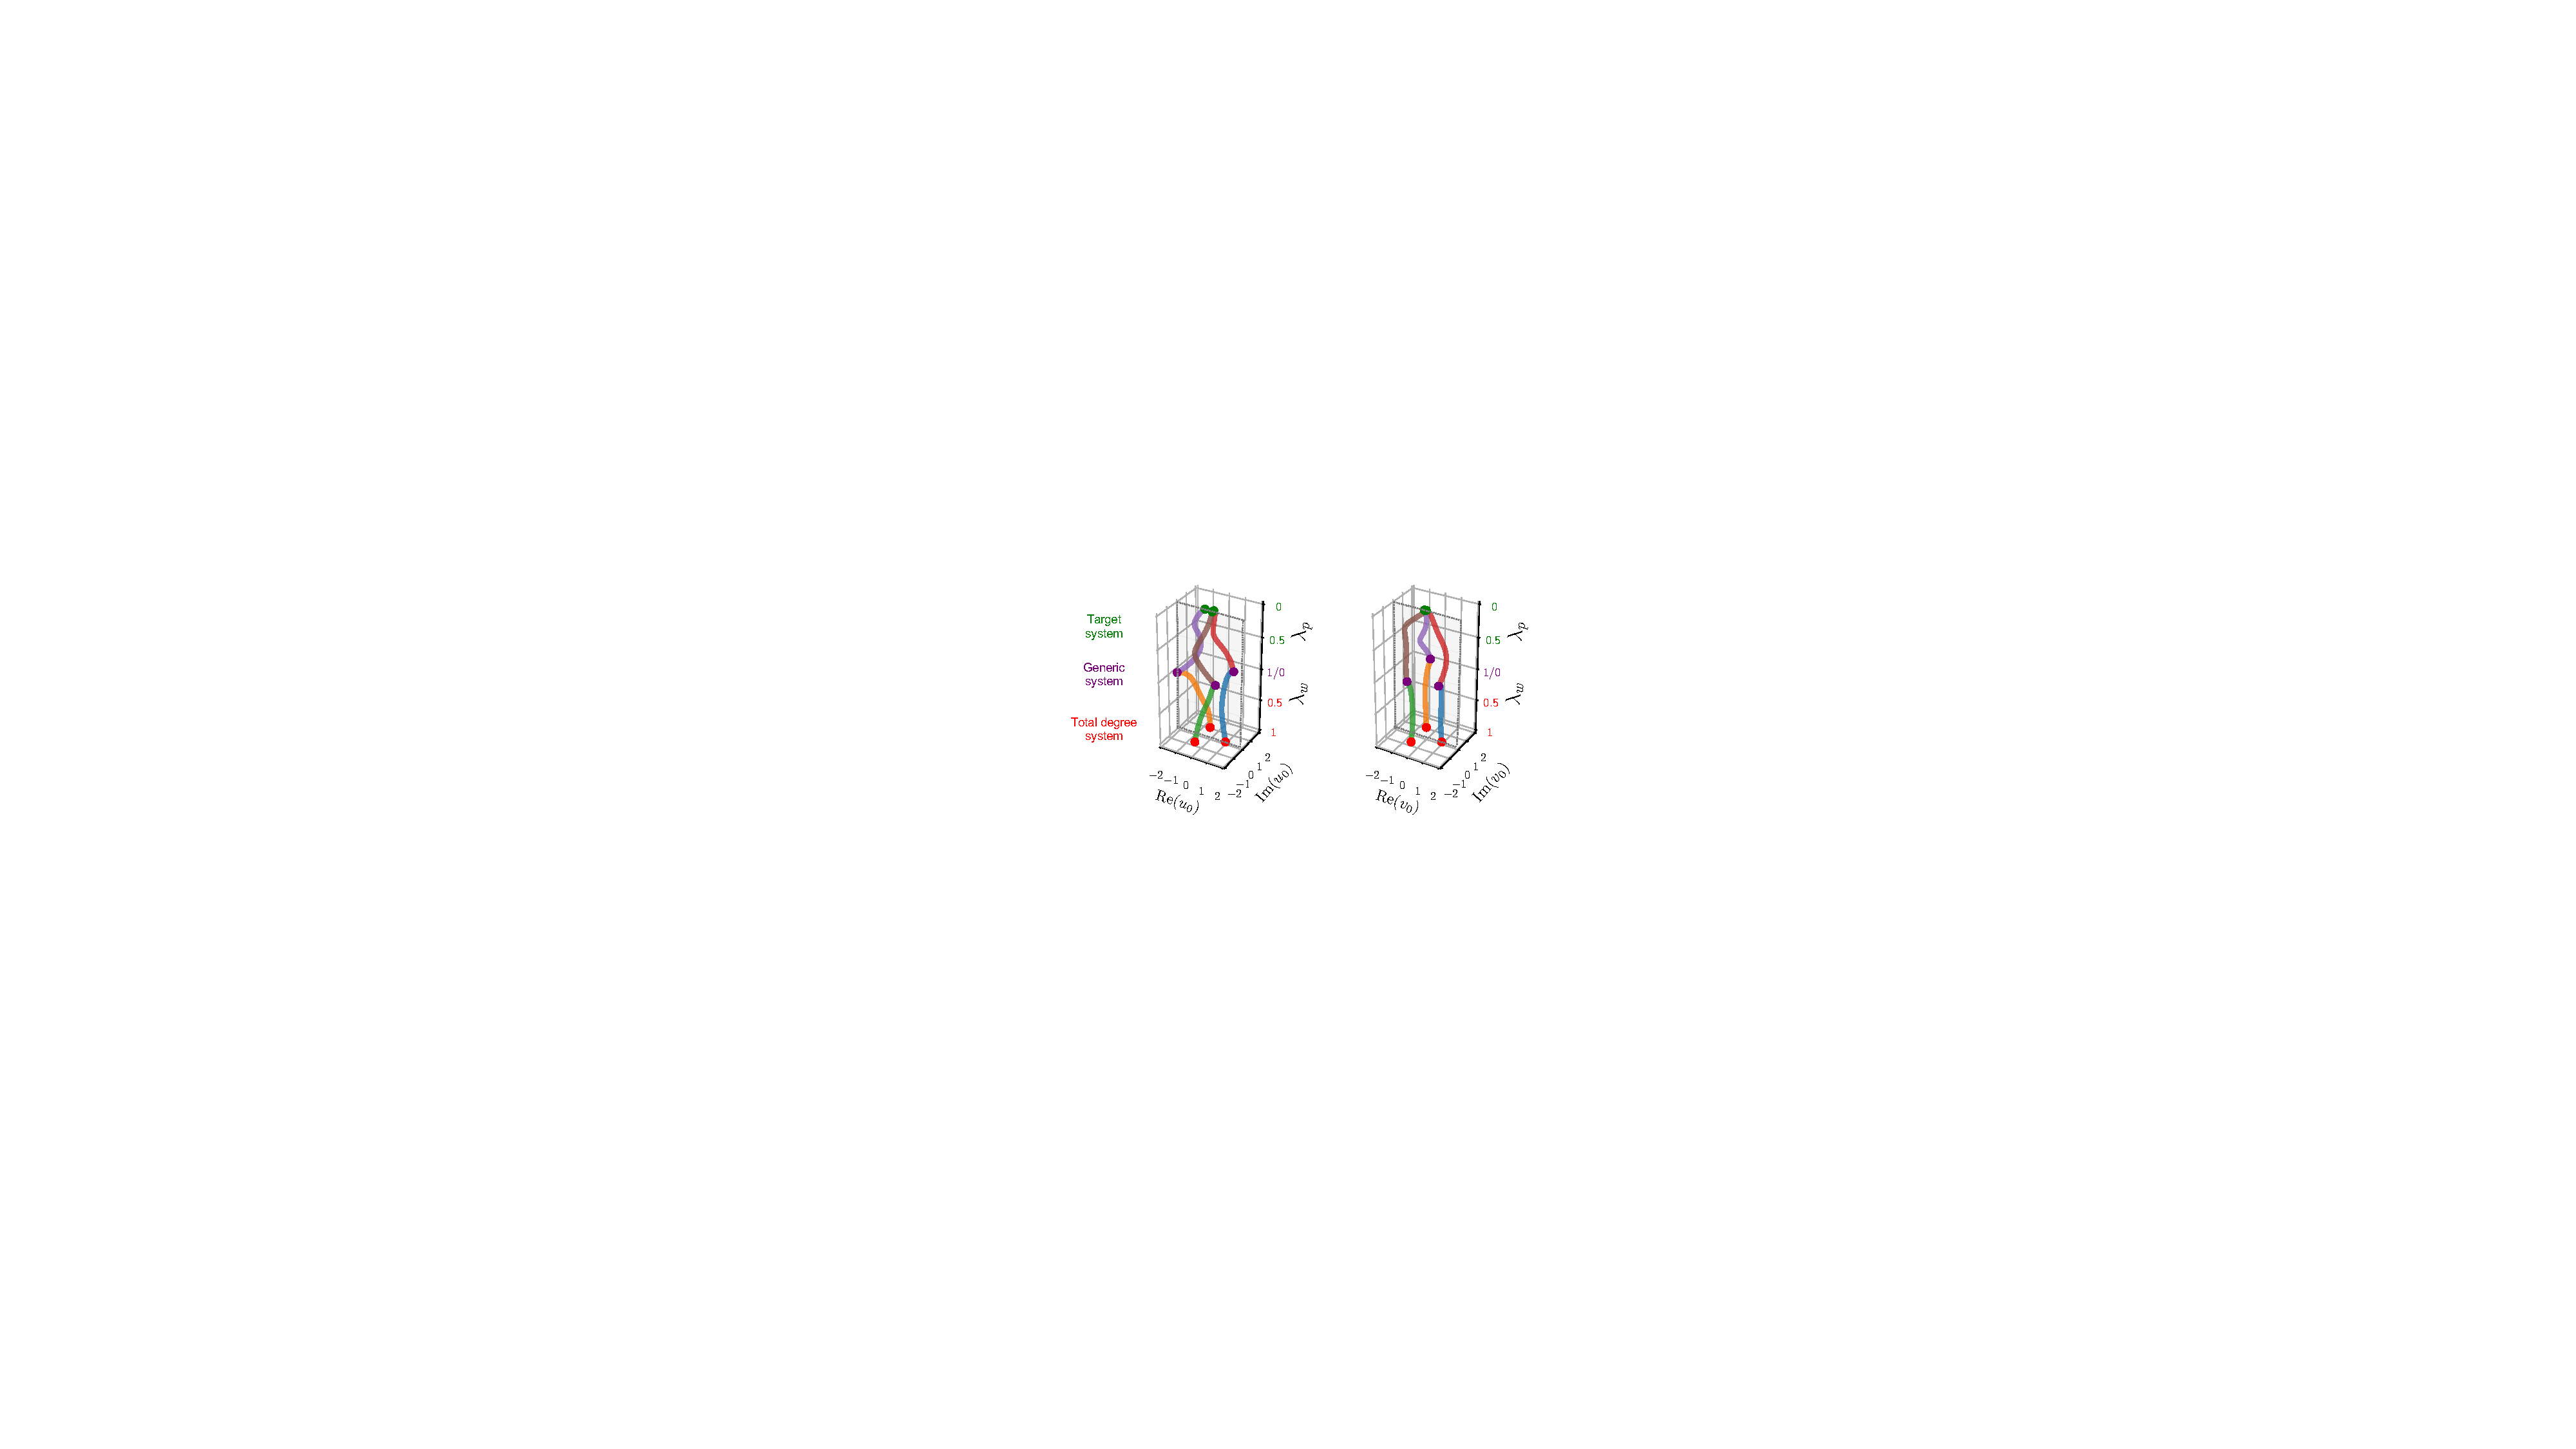
\includegraphics[width=\textwidth]{figures/hb/hb_paths.pdf}
	\caption{Homotopy continuation for the harmonic equations of a driven Duffing resonator (see Appendix \ref{app:harmeqs_11}). Path tracking from the complex roots of the system $\{u_0^3-1=0,v_0^3-1=0\}$ (red dots) to the roots of the harmonic equations (green dots), denoted $\vb{U}_0=(u_0,v_0)$.  To track steady states for multiple system parameters, we carry out a two-step process involving an initial full tracking (deformation $\lambda_w\in(0,1)$), where singular paths (not shown) are filtered out to arrive at the generic system solutions. This is followed by a tracking to the specific harmonic balance equations (deformation $\lambda_p\in(0,1)$), different for each set of system parameters.  The roots $\vb{U}_0$ traverse the complex plane until paths intersect with the planes $\mathrm{Im}(u_0)=0$ and $\mathrm{Im}(v_0)=0$ (light grey), at the 3 real roots of $\vb{\bar{G}}(\vb{U}_0)$. For this figure $\alpha=1$, $\omega_d=1.03$, $\omega_0=1$, $F=0.01$, and $\gamma=0.01$.}
	\label{fig:path_track}
\end{figure} 

HarmonicBalance.jl solves the algebraic Eq.~\eqref{eq:harmonic_balance} using the homotopy continuation method~\cite{Bates_2013, Verschelde_1999} as implemented by the open-source package HomotopyContinuation.jl~\cite{Breiding_2018}. To find the roots of a polynomial, this method starts from another polynomial of the same order, which is analytically solvable and saturates the Bézout bound. For instance, to find the roots of a single, $p$-th order polynomial $P(z)$ of a variable $z$, one can start from the polynomial $U(z)=z^p - 1$ with roots $e^{2\pi i k /p}$ ($k = 1,..., p$). Employing the so-called \textit{total-degree homotopy}, the polynomial $U(z)$ is gradually deformed\footnote{Here the homotopy is a mapping $H(U(z),P(z),\lambda)=\lambda U(z)+(1-\lambda)P(z)$, with deformation parameter $\lambda$, such that $H(U(z),P(z),\lambda=1)=U(z)$ and $H(U(z),P(z),\lambda=0)=P(z)$.} into the polynomial $P(z)$, correcting the known roots after each step, see Fig.~\ref{fig:path_track}. At the end of the homotopy continuation, the obtained set of roots is guaranteed to be complete, as it has been tracked from the full set of $p$ complex roots of $U(z)$.

Generalisation to multiple variables enables solving Eq.~\eqref{eq:harmonic_balance} by tracking the roots of the uncoupled system  $\{u_1^{d_1} - 1,v_1^{d_2} - 1,u_2^{d_3} - 1,v_2^{d_4} - 1,\cdots\}$, with $d_r$ equal to the degree of the polynomial $\bar{G}_r(\vb{U}_0)$, to those of $\bar{\vb{G}}(\vb{U}_0)$ (here $r=1,2,\ldots,2NM$ is an index labelling the harmonic equations). Such an approach leads to a number of solution paths to track that scales exponentially with $NM$. This constitutes a challenge in exploratory research that analyses the behaviour of the solutions as parameters vary. Crucially, in physical problems, $\bar{\vb{G}}(\vb{U}_0)$ often displays a vastly smaller number of roots than the B\'{e}zout bound. This implies that many of the solution paths are typically irrelevant since they do not lead to roots of $\bar{\vb{G}}(\vb{U}_0)$.
%This fact is leveraged by the solver algorithm used by HarmonicBalance.jl. 

It is important to mention here that although the obtained solutions are complex, only the real roots of Eq.~\eqref{eq:harmonic_balance} are physically meaningful. This may at first sight seem suboptimal -- why solve a large polynomial system if some solutions end up discarded? Indeed, the harmonic ansatz \eqref{eq:hb_ansatz} is commonly encountered in a complex form,
\begin{equation} \label{eq:hb_ansatz_a}
x_j(t) = \sum_{k=1}^M a_{j,k}(T) \e^{i \omega_{j,k} t } + \text{c.c} \,,
\end{equation} 
which is equivalent to Eq.~\eqref{eq:hb_ansatz} with $u_{j,k} = 2 \re{a_{j,k}}$ and $v_{j,k} = 2 \im{a_{j,k}}$. Upon applying the procedure detailed above, Eq.~\eqref{eq:hb_ansatz_a} yields a set of $MN$ equations for $\{ a_{j,k}\}$. In this case, complex solutions are physically sound. However, the method of homotopy continuation seeks the roots of a set of polynomials; the equations obtained from ansatz \eqref{eq:hb_ansatz_a} will typically contain complex conjugates of $\{ a_{j,k}\}$. For such equations, the B\'{e}zout theorem and subsequently the method of homotopy continuation cannot be used. HarmonicBalance.jl therefore operates exclusively with the real form \eqref{eq:hb_ansatz}.  

For a more detailed description of the homotopy continuation method and its implementation, see the documentation of HomotopyContinuation.jl and references therein~\cite{Sommese2005,Breiding_2018,timme2021numerical}. 

\subsection{Example: a driven membrane} \label{sec:hb_mem_driven}
We now come back to the example of a rectangular membrane whose equations of motion we found in Sec.~\ref{sec:hb_membrane_eom}. Suppose a periodic force drives it with frequency $\omega$. We now need to choose (i) which of the membrane modes we shall model and (ii) their corresponding harmonic ansatz [see Eq.~\eqref{eq:hb_ansatz}]. The main consideration here is which mode is closest to resonance. Let us assume a drive that is near-resonant with the fundamental mode frequency $\omega_{(1,1)} \equiv \omega_1$. We will denote this mode's amplitude by $x$ and use a single-harmonic ansatz based on the drive frequency $\omega$,
\begin{equation} \label{eq:hb_rect_ansatz0}
x(t) = u(T) \cos(\omega t) + v(T) \sin(\omega t) \,.
\end{equation}
The mode obeys the equation of motion
\begin{equation} \label{eq:hb_mem_eom1}
\ddot{x} + \gamma_1 \dot{x} + \omega_1^2 x + \alpha_{1111} x^3 = \cos(\omega t) \int_S \phi_{(1,1)} dS \equiv F_x \cos(\omega t)\,,
\end{equation}
where, in the notation of Eq.~\eqref{eq:hb_rect_eom}, $\alpha_{1111} = \alpha\, C_{\vb{jjjj}}$ with $\vb{j} = (1,1)$. We have also added a linear damping coefficient $\gamma_{1}$, which is usually phenomenological. 
Eq.~\eqref{eq:hb_mem_eom1} is known as the \textit{Duffing equation}. We will use it repeatedly in the subsequent Chapters to demonstrate various phenomena. 

To solve for steady states, we use the framework detailed in Sec.~\ref{sec:hb} to obtain and solve the harmonic equations (shown in Appendix \ref{app:harmeqs_11}). In Fig.~\ref{fig:hb_Duffing}, we show the resulting steady-state solutions, which show the most notable hallmark of a nonlinear system -- \textit{multistability}. In the region above $\omega \cong 1.03$, more than one steady-state response is possible. Which one the system chooses depends on the initial conditions.
\begin{figure}
	\centering
	\includesvg{figures/hb/11.svg}
	\caption{Steady state solutions of the Duffing equation, using the single-harmonic ansatz \eqref{eq:hb_rect_ansatz0}. Colours denote the three branches, stable (full) and unstable (dotted) solutions are distinguished using the methods of Chapter \ref{ch:linresp}. Parameters used: $\omega_0 = \alpha = 1, \, \gamma = 0.01,\,F = 0.01$. The code used to generate this data is shown in Appendix \ref{sec:app_duffing_example}.}
	\label{fig:hb_Duffing}
\end{figure}

\subsubsection{Harmonic selection}

Eq.~\eqref{eq:hb_mem_eom1} represents a perfectly valid approach to find the response of the fundamental mode~\cite{Steeneken_2021, Miller_2021}. However, exciting the system with frequency $\omega$ causes, to first order, a frequency conversion $\omega \rightarrow 3\omega$ by the cubic nonlinearity. Although we could add $3\omega $ to the harmonic ansatz of $x$, this motion is far off the mode's resonance and will typically be negligible. On the other hand, the membrane system offers additional modes to be excited, notably the (3,3) mode, which is nonlinearly coupled to (1,1) (see the selection rules in Sec.~\ref{sec:hb_membrane_eom}), and has triple its natural frequency, $\omega_{(3,3)} \equiv \omega_3 = 3 \omega_1$. Denoting its amplitude by $y(t)$, we choose the ansatz
\begin{equation} \label{eq:hb_1133_ansatz}
x(t) = u_1(T) \cos(\omega t) + v_1(T) \sin(\omega t) \,, \quad y(t) = u_2(T) \cos(3\omega t) + v_2(T) \sin(3\omega t) \,.
\end{equation}
Note that not only the $3\omega$ harmonic of $x$ is neglected, but so is the $\omega$ harmonic of $y$. The two modes obey the equations of motion, again adding linear damping,
\begin{equation} \label{eq:hb_mem_2mode}
\begin{gathered}
\ddot{x} + \gamma_1 \dot{x} + \omega_1^2 x + \alpha_{1111} x^3 + \alpha_{1133} x y^2 + \alpha_{1113} x^2 y = F_1 \cos(\omega t)\,, \\
\ddot{y} + \gamma_3 \dot{y} + \omega_3^2 y + \alpha_{3333} y^3 + \alpha_{1133} x^2 y + \alpha_{3111} x^3 = F_3 \cos(\omega t)\,,
\end{gathered} 
\end{equation}
where
\begin{equation}
F_1 = \int_S \phi_{(1,1)} dS\,, \quad F_3 = \int_S \phi_{(3,3)} dS \,.
\end{equation}
\begin{table}[ht] 
	\centering
	\caption{Relative magnitudes of the various nonlinear coupling terms seen in Eq.~\eqref{eq:hb_mem_2mode} obtained using Eqs.~\eqref{eq:hb_rect_eom} and \eqref{eq:hb_rect_C}, in the limit $L_x = L_y$.}
	\label{table:hb_rect_coeffs}
	\begin{tabular}{ |c|c| } 
		\hline
		term & coefficient \\ \hline
		$\alpha_{1111}$	& $1$ \\
		$\alpha_{3311} = \alpha_{1133}$ & $72/5$\\ 
		$\alpha_{3111}$ & $-3/5$ \\
		$\alpha_{1113}$ & $-9/5$ \\
		$\alpha_{3331}$ & $0$\\
		$\alpha_{3333}$ & $81$ \\ \hline
	\end{tabular}
\end{table}
%
\begin{figure}
	\centering
	\includesvg{figures/hb/11_33_ss.svg}
	\caption{Steady state solutions for the two-mode model [see Eq.~\eqref{eq:hb_mem_2mode}] under the ansatz \eqref{eq:hb_1133_ansatz}. Stable (full) and unstable (dashed) solutions were determined using the analysis presented in Sec.~\ref{sec:linresp}. Parameters used: $\omega_1^2 = (\omega_3/3)^2 = 1, \, \gamma_1 = \gamma_3 = 10^{-3},\, \alpha = 10^{-5}, \, F_1 = F_3 = 0.5 $. The code used to generate this data is shown in Appendix \ref{sec:app_duffing_example}.}
	\label{fig:hb_rect_ss1}
\end{figure} 
Although multiple nonlinear coupling terms now appear, only their overall scale is a free parameter -- their ratios are fixed as these all originate from the substrate nonlinearity $\alpha$ described in Sec.~\ref{sec:hb_membrane_eom}. In Table~\ref{table:hb_rect_coeffs}, we list the relevant coefficients in the limit of a square membrane.

Again, we obtain the harmonic equations (see Appendix \ref{app:harmeqs_1133}) and find steady states. For two coupled resonators with a cubic nonlinearity featuring one harmonic each, we arrive at a B\'{e}zout bound $3^4 = 81$ for the number of solutions. The resulting solution diagram, shown in Fig.~\ref{fig:hb_rect_ss1}, displays qualitatively new behaviour compared to the single-mode model, most notably a stable high-amplitude branch (shown in brown) disconnected from the other stable branches. We do not attempt an interpretation of the results here -- they serve to highlight the power of harmonic balance combined with homotopy continuation to analyse complicated multistable behaviour. In practice, the framework can be used to efficiently solve far larger systems, see Example \ref{sec:hopf_example} and Appendix \ref{app:hb}. 

\subsubsection{Nonlinear damping}

Dissipation is an inevitable occurrence in any physical system. We have so far modelled it with a linear damping coefficient. In practice, however, many systems show increased dissipation at high excitation amplitudes -- \textit{nonlinear dissipation}. Here, we model this effect\footnote{Under inversion symmetry, commonly present in experimental scenarios, only terms of odd powers in $x, \dot{x}$ may appear in the equations of motion.} by modifying the equations of motion with $\gamma_1 \rightarrow \gamma_1 + \eta_1 x^2$ and $\gamma_3 \rightarrow \gamma_3 + \eta_3 y^2$. The resulting steady states for the two-mode system are shown in Fig.~\ref{fig:hb_duff_nld}. We see that the addition of nonlinear dissipation terminates the high-amplitude branches. In real systems, however, this effect may be far weaker, and the branches may stretch across a large $\omega$ range~\cite{Yang_2021a}. 
\begin{figure} [h!]
	\centering
	\includesvg{figures/hb/11_33_ss_nld.svg}
	\caption{Steady-state solutions for the two-mode model shown in Fig.~\ref{fig:hb_rect_ss1} after adding nonlinear damping $\eta_1 = \eta_3 = 5\cross 10^{-7}$.}
	\label{fig:hb_duff_nld}
\end{figure} 

\section{Heuristic methods for nonlinear damping}

We have seen that adding nonlinear damping to our system caused qualitative changes in its behaviour. Due to the effective lowering of the quality factor, nonlinear damping is also detrimental to potential applications of nonlinear resonators~\cite{Catalini_2021, Kosata_2020}. Its origins are, however, not always clear~\cite{Bachtold_2022, Steeneken_2021}. Detailed works exist which analyse system-specific phenomena such as thermoelasticity~\cite{Atalaya_2016, Cleland} and viscosity of a surrounding medium~\cite{Aureli_2010}. 

In systems with multiple modes present, a geometric nonlinearity, such as the one introduced in Sec.~\ref{sec:hb_membrane_eom}, can cause undesired coupling of the modes. This effect has been identified as a possible source of nonlinear damping~\cite{Kecskekler_2021, Guttinger2017, Dykman_1975}. Here, we present an analytically treatable example derived from the two-mode model analysed in Sec.~\ref{sec:hb_mem_driven}. We confirm that nonlinear damping appears in that system and suggest an experimental method for its reduction. 

\subsubsection{High-harmonic generation}

Let us revisit the two-mode model introduced in Eq.~\eqref{eq:hb_mem_2mode}, where a mode $x(t)$ is coupled to another mode, $y(t)$, via a cubic nonlinearity. If only the mode $x(t)$ is driven\footnote{This holds by construction since the drive frequency $\omega$ appears in the ansatz for $x(t)$ but for $y(t)$ in Eq.~\eqref{eq:hb_1133_ansatz}.} and the coupling is weak, we may assume the amplitude of $y(t)$ is small and leave out any terms nonlinear in $y(t)$. Keeping the notation of Sec.~\ref{sec:hb_mem_driven}, 
\begin{equation} \label{eq:hb_nld_eom}
\begin{gathered}
\ddot{x}(t) + \gamma_1 \dot{x}(t) + \omega_1^2 x(t) + \alpha_{1111} x(t)^3 +  3 \alpha_{3111} x(t)^2 y(t) = F_1 \cos(\omega t) \,, \\
\ddot{y}(t) + \gamma_3 \dot{y}(t) + \omega_3^2 y(t) + \alpha_{3111} x(t)^3 = 0 \,.
\end{gathered}
\end{equation}
In this particular example, it is advantageous to use the complex form of the harmonic ansatz introduced in Eq.~\eqref{eq:hb_ansatz_a},
\begin{equation}
x(t) = a(T) \e^{i \omega t} + \text{c.c.} \,, \quad y(t) = b(T) \e^{3 i \omega t}  + \text{c.c} \,.
\end{equation}
Collecting the prefactor of  $e^{i \omega t}$ in the first equation, we obtain
\begin{equation} \label{eq:hb_nld_A}
\left(- \omega_1^2 + i \gamma_1 \omega + \omega_1^2\right) a + 3\alpha \abs{a}^2a + 3 (a^*)^2 b = F_1/2 \,,
\end{equation}
and similarly for $e^{3 i \omega t}$ in the second equation, 
\begin{equation} \label{eq:hb_nld_B}
b = \frac{a^3}{(3\omega)^2 - \omega_3^2 - 3 i \gamma_3 \omega} \,.
\end{equation}
Note that we are \textit{not} attempting a full solution here since, as explained in Sec.~\ref{sec:hb}, nonlinear equations of motion are usually not analytically solvable. However, since the problem is linear in $b$, we may combine Eqs.~\eqref{eq:hb_nld_A} and \eqref{eq:hb_nld_B} to get
\begin{equation} \label{eq:hb_nld_selfcons}
a = \frac{F_1}{2} \left[\omega_1^2 - \omega^2 + 3 \alpha \abs{a}^2 + \re{K} \abs{a}^4  + i \left( \gamma_1 \omega +  \im{K} \abs{a}^4 \right)\right]^{-1} \,,
\end{equation}
with $K = \frac{3 \alpha_{3111}^2}{(3\omega)^2 - \omega_3^2 - 3 i \gamma_3 \omega}$.
Although unsolvable analytically, Eq.~\eqref{eq:hb_nld_selfcons} does offer some insight. The real part of the brackets on the right-hand side describes the resonance condition. In a fully linear problem, $\alpha_{1111} = \alpha_{3111} = 0$ and the response is maximised for $\omega = \omega_1$. The Duffing self-nonlinearity $\alpha_{1111}$ causes an effective shift of the resonance frequency, as does $\re{K}$. More importantly, $\im{K}$ enters the equation alongside the linear damping coefficient $\gamma_1$. We hence observe that $\gamma_1$ is renormalised to $\gamma_1^{\rm nl}$,
\begin{equation} \label{eq:nld_gamma}
\gamma_1^{\rm nl} = \gamma_1 + \frac{1}{\omega} \im{K} \abs{a}^4 = \gamma_1 + \frac{3 \gamma_3 \alpha_{3111}^2 \abs{a}^4}{( 9\omega^2 - \omega_3^2)^2 + 9 \gamma_3^2 \omega^2} \,,
\end{equation}
so that the mode $x(t)$ displays effective nonlinear damping. 

\subsubsection{Thermal excitations}

Eq.~\eqref{eq:nld_gamma} shows quartic dependence of the nonlinear damping coefficient on $\abs{a}$. However, phenomenological models of this effect, such our two-mode model in Sec.~\ref{sec:hb_mem_driven}, typically assume quadratic dependence, as this is the lowest order that respects inversion symmetry. Moreover, in practice, nonlinear damping is often temperature dependent~\cite{Catalini_2021}, which hints at thermal excitations being a possible culprit. Here we give an impression of how thermal excitations affect our model above; a comprehensive treatment of the necessary methods can be found in Refs.~\cite{Gardiner, Roberts_1986, Khasminskii_1966, Toni_thesis}.

Allowing for nonzero temperature, both amplitudes $a$ and $b$ can be written as a sum of deterministic terms, $a_0$ and $b_0$, and stochastic terms induced by thermal noise, $\delta a$ and $\delta b$,
\begin{equation}
a = a_0 + \delta a \,, \quad b = b_0 + \delta b \,. 
\end{equation} 
Although the stochastic terms are by definition unknown, their statistical properties are fixed. In particular, the phase fluctuations of thermal motion give $\expval{\delta a^n} = 0$ for all integer $n$, while $\expval{ \abs{\delta a}^2} \propto T $ since this is proportional to thermal energy, as per the fluctuation-dissipation theorem. To now quantitatively determine the effect of nonzero temperature on $a$, we would need to adapt the method of harmonic balance to stochastic excitations, which may be done using the method of \textit{stochastic averaging}~\cite{Roberts_1986, Khasminskii_1966, Toni_thesis}. Here we do not pursue this direction further but note that considering the statistical properties given above, one arrives at $\expval{\abs{a^4}} = \abs{a_0}^4 + 6 \abs{a_0}^2 \expval{ \abs{\delta a}^2} + \expval{\abs{\delta a}^4}$. Inserting this into Eq.~\eqref{eq:hb_nld_selfcons} results in a temperature-dependent damping coefficient, which shows a square dependence on $\abs{a_0}$.
\subsection{Removal by feedback control} \label{sec:hb_damping_the_damping}

The mechanism of nonlinear damping via an auxiliary mode $y$ has a surprising consequence. When $y$ is highly dissipative, $\gamma_3$ becomes the dominant term in Eq.~\eqref{eq:nld_gamma}. In this limit, $\gamma_1^{\rm nl}$ tends back towards the linear damping coefficient, $\gamma_1^{\rm nl} = \gamma_1$. Despite making the system more dissipative, we seem to have removed the effective nonlinear damping.

The phenomenon can be explained intuitively. The damping coefficient $\gamma_3$ corresponds to a force $F_{d} = - \gamma_3 \dot{y}$ opposing the motion of $y$, which causes energy dissipation at a rate linearly proportional to the amplitude $\abs{b}$. However, in the limit of $\gamma_3 \rightarrow \infty$, we have $ \abs{b} \propto 1/\gamma_3$.
The energy dissipated by $y$ during one period $\tau$ of the system
\begin{equation}
\Delta E = -\int_{y(0)}^{y(\tau)} \gamma_3 \dot{y} \, dy = -\int_0^\tau \gamma_3 \dot{y}^2  \, dt\propto \gamma_3 \abs{b}^2 \propto 1 / \gamma_3\, ,
\end{equation}
so that at $\gamma_3 \rightarrow \infty$, the energy loss via this channel vanishes. 

Besides being an insightful demonstration, this phenomenon may have a practical application. In many experimental setups (see Chapter \ref{ch:spins}), the so-called \textit{feedback damping} is used, which employs a very fast tracking of an oscillator by a lock-in amplifier in order to exert a force opposing its velocity. Feedback-damping the motion at frequency $\omega$ hence effectively increases $\gamma_1$ -- enhancement by many orders of magnitude is routinely achieved~\cite{Courty_2001, Kleckner_2006, Poggio_2007, Rossi_2018}.
Feedback-damping instead the motion at $3\omega$ would effectively increase $\gamma_3$, thus eliminating the nonlinear dissipation pathway. To our knowledge, an experimental demonstration of such "damping of the damping" is yet to be seen. 
